% memory-bench: dataset, construction methodology, and validity study.
% arXiv preprint format (single column). Self-contained: all figures are TikZ /
% pgfplots, no external image files.
%
% Every number in this file traces to a committed artifact; the mapping is
% asserted by tests/test_paper_numbers.py and tests/test_paper_tex.py.

\documentclass[11pt]{article}

\usepackage[margin=1.1in]{geometry}
\usepackage[T1]{fontenc}
\usepackage{lmodern}
\usepackage{microtype}
\usepackage{amsmath}
\usepackage{amssymb}
\usepackage{booktabs}
\usepackage{array}
\usepackage{caption}
\usepackage{enumitem}
\usepackage{tikz}
\usepackage{pgfplots}
\usepackage[hidelinks]{hyperref}

\pgfplotsset{compat=1.18}
\usetikzlibrary{positioning, arrows.meta, fit, backgrounds,
                decorations.pathreplacing, calc}

\captionsetup{font=small, labelfont=bf, width=.95\textwidth}

% Tufte-leaning plot defaults: no frame, no grid, minimal ticks. Every rule
% that survives here is carrying information.
\pgfplotsset{
  tufte/.style={
    axis lines=left,
    axis line style={draw=black!55, line width=.4pt},
    tick style={draw=black!55, line width=.4pt},
    tick align=outside,
    label style={font=\small},
    tick label style={font=\footnotesize},
    legend style={draw=none, fill=none, font=\footnotesize},
    every axis plot/.append style={line width=.9pt},
  },
}

\definecolor{ink}{gray}{0.15}
\definecolor{mid}{gray}{0.50}
\definecolor{pale}{gray}{0.78}
\definecolor{accent}{RGB}{176,48,36}

\newcommand{\code}[1]{\texttt{\small #1}}

\title{\textbf{memory-bench}\\[.3em]
\large A Screened Benchmark Dataset and Validity Study for\\
Organizational Memory in Agent Harnesses}

\author{Mehul Srivastava\\\normalsize Independent}

\date{14 September 2026}

\begin{document}
\maketitle

\begin{abstract}
\noindent
An organization's agents no longer run on one model: each person picks the
harness built for their work, and picks it \emph{because} it is specialized. The
weights organizational knowledge must reach are therefore plural and
vendor-owned, so coherence cannot live in them. The memory layer is the only
place every harness can reach. Of the ten published memory benchmarks we
verified (\S2), none measures whether a memory system holds that knowledge with
the right scope, authority, and freshness.

We release memory-bench, an instrument for that question, with the evidence that
it measures what it claims. The dataset is three simulated software
organizations: multi-week event streams delivered event-by-event to each
principal who witnessed them, a hidden ground-truth ledger, and behavioral work
tasks injected at evaluation time rather than quiz questions. Every probe
instance is paired with a counterfactual twin in which the probed fact differs
and the rest of the stream is byte-identical; an instance is credited only when
both sides pass, so an answer available from prior knowledge earns nothing.
Across three seeds, 371 instances survive a five-gate screening pipeline under
blinded judging; two further seeds are withheld unscreened as holdouts.

The validity study is this paper's result. A memoryless worker's pair credit is
statistically indistinguishable from zero on every capability rung, which is
direct evidence that the design does not reward priors. Probe validity is
\emph{task-model-relative}: under identical strict rules, 37/54 probe clusters
survived the ceiling gate for one worker and 17/54 for a smaller sibling. The
harness is part of the consumer: identical weights behind two agent harnesses
agreed on only 65\% of twin-ceiling outcomes, failing a prespecified 90\% bar.
Judge--human agreement on a blinded 150-pair packet reached 81.3\% raw agreement
at $\kappa = 0.537$, which \textbf{fails} our prespecified gate of $\kappa \geq
0.75$. Aggregate disagreement is symmetric, 14 items each way, but that symmetry
is a cancellation rather than a property of the judge: every one of its errors on
absence-phrased criteria is an over-accept (8 of 8; it returns \textsc{false} on
1 of 44 such items), and every one of its errors on scope criteria is an
under-accept (7 of 7). Our cheaper automated check, a 20-decoy false-accept
audit, passed this same judge at 2/41 and could not have caught the defect: none
of those 41 criteria were absence-phrased. The mechanism does not depend on the
human labels. Across all 5{,}398 committed criterion verdicts the absence class
passes at 96.4\% against 39.0\% and 36.9\% for the other two kinds, and under a
memoryless worker, where the other two roughly halve, it holds at 96.2\%,
unmoved by removing the very knowledge the instrument measures. The transferable
lesson is to report judge agreement per criterion type, because an aggregate
false-accept rate can conceal opposite directional failures that cancel.

Mid-study, the provider deprecated the pinned worker, which ended comparative
evaluation and exposed a dependency every agentic benchmark carries and few
state: screening anchors are properties of a worker, not of the data. We report
the event, release the partial rows as provenance, and specify the re-anchoring
procedure that lets the dataset outlive any single worker. No comparative system
result is claimed anywhere in this paper.
\end{abstract}

\section{Introduction}

\subsection{Organizational knowledge has no home in the weights}

Organizations are getting smaller while the number of agents working inside them
grows, and the agents are not interchangeable. A developer's coding agent, a
designer's creative tool, and a generalist assistant differ in system prompt,
tools, and defaults, and each is chosen for those differences. This heterogeneity
is a property of the ecosystem rather than a transitional untidiness to be
standardized away.

One structural consequence follows. If the weights an organization runs on are
plural and vendor-owned, then organizational coherence cannot live in them. The
decisions, working rules, preferences, and commitments that make a company act
like one company have to be held somewhere every harness can reach, and the
memory layer is the only such place. On this view a memory system is not an
accessory to an organization's agents; it is the connective tissue.

The naive version of that idea does not work. Pooling every artifact and giving
every agent the same view produces a rumor mill with perfect recall, not a
collective intelligence. A personal preference is not org policy. A leadership
decision outranks a loud opinion. A superseded plan must stop driving behavior
while remaining retrievable. A need-to-know fact must not diffuse. What makes an
organizational world model useful is that it is \emph{scoped, tiered, and
temporally correct}: each agent receives the context appropriate to its principal
and its task, at the current epoch of truth.

\subsection{What existing benchmarks measure instead}

Published memory benchmarks overwhelmingly evaluate a single agent's recall over
a long conversation: can the system retrieve a fact it was told earlier. That is
rung 0 of the capability ladder this benchmark is organized around (\S3.3), it is
table stakes, and long context saturates it. Organizational memory differs along
three axes that single-agent recall does not exercise: events have multiple
witnesses and per-principal visibility, facts carry tier and authority so that
conflicts have correct rather than arbitrary resolutions, and facts are
invalidated over time rather than merely accumulated.

The gap is not only in coverage. Section~2 surveys the field's measurement
failures: answers guessable from priors, corpora answerable without memory at
all, corrupted ground truth producing impossible ceilings, judges that accept
topical waffle, protocols loose enough to support score disputes between vendors.
These are the reasons this paper spends most of its length on validity rather
than on results.

\subsection{What we claim, and what we do not}

This paper claims an \emph{instrument}, not a leaderboard.

We claim that the released dataset measures organizational memory behavior at
rungs 1--3 of the ladder, for a two-team simulated software organization at
L1--L2 scale, under a stated worker pin; and we report the measurements that
support or qualify that claim, including the ones that qualify it. We do not
claim that any memory system is better than another. This paper publishes no
comparative system numbers. We do not claim to measure ``mini-AGI-ness,'' and the
external-validity claim stops at the organization type instantiated. No result is
ever reduced to a single aggregate score: results are grouped by capability rung,
always.

Three constraints were fixed before the evidence they govern was produced, and
each is corroborated by dated git history rather than by assertion: the gate
criteria and scoring rules, the worker and judge pins, and the commitment to
carry failed gates as failures rather than repairing the probes that failed them.
That commitment has a visible price in this paper. \textbf{All three released
seeds fail the instance gate} (125, 131, and 115 valid instances against a
threshold of 135), and \textbf{seed 3's cluster gate also fails} (40/54 surviving
clusters). The instances are retained, marked, and reported as failures rather
than topped up, because a gate that is relaxed once it binds was never a gate.

\subsection{Contributions}

\begin{enumerate}[leftmargin=*, itemsep=.35em]
\item \textbf{A screened dataset} (\S3): 371 valid paired probe instances across
three simulated organizations, with counterfactual twins, hidden ground-truth
ledgers, and two unscreened holdout seeds. Every gate result is dated and
corroborated by commit history.

\item \textbf{A construction and screening methodology} (\S3): pair credit via
counterfactual twins; per-item floor and ceiling validity screening with a pinned
worker; blinded judging with a versioned rubric where the judge model is never
the worker model nor the family that authored the criteria; a five-gate pipeline;
and a statistics protocol prespecified before any result existed.

\item \textbf{A validity study} (\S4): the measurements that test whether the
instrument works: floor validation, the task-model-relativity of probe validity,
harness sensitivity, judge false-accept rate, and judge--human agreement.

\item \textbf{A durability procedure} (\S4.6): what it takes to keep an agentic
benchmark valid when the worker it was screened under disappears. We did not
choose this contribution; the provider deprecated our pinned worker mid-study and
we documented what that costs and how to recover from it.
\end{enumerate}

\subsection{What this paper does not contain}

It contains no system comparison. The pilot that would have produced one had
completed the memoryless floor condition and partial rows for four further
baselines when the pinned worker became unreachable through every available
billing path (\S4.6). Because probe validity is worker-relative (\S4.2),
attaching a new worker's results to anchors measured under the old one would
break both the normalization and the pair-validity argument, so we did not do it.
The partial rows are released in \S6 as provenance for an interrupted
prespecified pilot, carrying no comparative claim.

\section{Related work}

\noindent\textit{Citation note.} Every reference in this section was resolved
against its primary source on 2026-09-14, because the section was first drafted
from this project's own field audit rather than from the papers. All twenty
arXiv identifiers resolve to a paper matching the name given, including the six
that postdate the drafting model's knowledge, and a deliberate nonexistent
identifier was checked to confirm that failures report as failures. Three
descriptions were wrong and are corrected here, and one claim was refuted by its
own source and rewritten rather than re-cited.

\subsection{What memory benchmarks currently measure}

The established memory benchmarks evaluate one agent's recall across a long
conversation. LoCoMo (arXiv 2402.17753) and LongMemEval (2410.10813) ask whether
a system can retrieve a fact stated in an earlier session, sometimes with a
temporal qualifier, and MemBench (2506.21605) extends the format. These are
rung-0 tasks: recall on request, which is table stakes for a memory system and
which long context saturates.

A second line moves toward agentic settings. MemoryAgentBench (2507.05257)
argues that pasting a conversation history into context evaluates memory
off-policy, since a deployed system writes its memory incrementally rather than
receiving the whole history at once. MemoryArena (2602.16313) evaluates
closed-loop single-principal agentic tasks. StreamMemBench (2606.14571) covers
streaming ingestion of egocentric lifelog data and feedback consolidation, and
HorizonBench (2604.17283) covers personal preferences that change over time.
LongMemEval V2 (2605.12493), despite the name, is a different object from the
original: a web-agent benchmark over trajectories reaching 115M tokens, scoring
static state recall, dynamic state tracking, workflow knowledge, environment
gotchas, and premise awareness. Each of these remains single-principal.

Two works are close enough that the distinction has to be drawn precisely rather
than by category.

MEMTRACK (2510.01353) is the nearest neighbour on the organizational axis, and it
is not a conversational benchmark at all. It models realistic organizational
workflows by interleaving asynchronous events across Slack, Linear, and Git, with
noisy, conflicting, and cross-referring information, and it scores acquisition,
selection, and conflict resolution rather than retrieval alone. Its best reported
model reaches 60\% correctness. Anyone reading our framing should read MEMTRACK
first. What separates it from this work is not ambition but structure: MEMTRACK
is single-agent, so it has no witness model and no notion of a fact reaching one
person and not another. It scores conflict resolution without tiered authority
deciding which side of a conflict is correct, and without supersession as a
distinct failure mode from retrieval.

GateMem (2606.18829) is the nearest neighbour on the multi-principal axis,
evaluating memory governance for shared-memory agents across utility, access
control, and deletion. It shares our premise that a memory system serving several
people is a different object from one serving a single user. It scores access
control on its own; we score governance jointly against propagation, because the
two pull in opposite directions and a system can win either by sacrificing the
other. That tension is the reason v1 defers leakage scoring rather than reporting
it alone.

\subsection{Why organizational memory is a different object}

Single-agent recall does not exercise three properties that decide whether an
organization's agents behave coherently.

\textbf{Events have witnesses.} In a conversation benchmark every turn is visible
to the one agent under test. In an organization a decision made in a meeting
reaches the people in the room, and whether it reaches anyone else is the
question being asked. Our streams are delivered per principal according to a
witness model, so a system that pools everything and a system that respects
visibility see different inputs by construction (\S3.2).

\textbf{Facts carry authority and tier.} When a personal preference contradicts a
team convention, or a loud opinion contradicts a leadership decision, there is a
correct answer rather than an arbitrary one. Recall benchmarks have no notion of
a fact outranking another fact, so they cannot score getting it wrong.

\textbf{Facts are invalidated, not only accumulated.} A superseded plan must stop
driving behavior while staying retrievable on request. A benchmark that scores
retrieval alone credits a system for surfacing a fact that should no longer
apply.

Continual-learning and knowledge-editing work addresses the third property inside
the weights. This benchmark takes the harness position instead: the knowledge an
organization runs on changes faster than anyone retrains, and the agents
consuming it run on models the organization does not own.

\subsection{How memory evaluations have failed in practice}

Most of this paper is validity evidence rather than results, and the reason is
that this field's published numbers have repeatedly failed on measurement rather
than on modeling.

An independent audit of LoCoMo (Penfield Labs, 2026-04-08) found 99
score-corrupting errors in 1{,}540 questions, roughly 6.4\%, putting a ceiling of
about 93.6\% on the benchmark while vendors published scores above it. The same
audit reported that an LLM judge accepted topical but wrong answers at 62.81\%.
The audit is self-published rather than peer-reviewed, and its author
independently discloses the same finding in a public issue thread, so the figure
has two routes rather than one.

The comparison that should carry the most weight comes from a vendor's own paper.
Mem0's evaluation (2504.19413, Table 2) reports a full-context baseline at
72.90\% against Mem0's graph variant at 68.44\% and plain Mem0 at 66.88\%. The
system's own published table shows the no-memory-system baseline winning, which
raises the question of whether the corpus needed a memory system at all. Letta
separately reported that a plain filesystem-and-grep agent reached 74.0\%. That
is why a grep agent is one of our registered baselines: a memory product should
have to beat a directory of files.

Protocol looseness produced a public scoring dispute between Mem0 and Zep, with
the same system reported at 84\%, then 75.14\%, then 58.44\% depending on
configuration and denominator. Neither party was obviously acting in bad faith,
which is the point: without one prespecified scoring rule and one denominator,
two honest groups produce different numbers. MemDelta (2606.29914) found that an
embedding-only swap shifted accuracy by 6.2 points ($p = 0.004$) while the
architectural comparison it ran, verbatim RAG against full context, was not
significant (47.2 against 49.8, $p = 0.34$). That is why our RAG-class baselines
pin and report their embedding model.

A separate failure is fitting the system to the test after seeing it. A public
teardown of MemPalace documents three patches hand-coded against three specific
questions the system had failed, a quoted-phrase boost, a person-name boost, and
a pattern match for two particular phrasings, after which the result was reported
as the first perfect score on LongMemEval. The reporter's summary is that the
fixes were designed around the exact failure cases rather than discovered by
analyzing general failure patterns. The same teardown records retrieval
parameters set beyond the size of the corpus being searched and a metric mismatch
against other systems' end-to-end numbers.

We should be precise about what this does and does not motivate, because an
earlier draft of this paragraph overstated it. The documented failure is test-set
inspection followed by targeted repair, not benchmark content being visible
during ingestion. It is an argument for a withheld ledger, for holdout seeds that
can be regenerated, and for a freeze that makes post-hoc repair visible in git
history, all of which this paper's design carries. The separate decision to
inject probes only at evaluation time comes from our own threat model rather than
from this source.

\subsection{Benchmark validity and benchmark decay}

Work on benchmark quality supplies the standards this paper is written against.
BetterBench (2411.12990) assesses benchmarks across their lifecycle and finds
statistical reporting the most commonly failed criterion; the Agentic Benchmark
Checklist (2507.02825) sets out validity requirements specific to agentic
evaluation, including auditing a scorer against degenerate strategies; and a
construct-validity audit of 445 benchmarks (2511.04703) documents how often a
benchmark's measured quantity differs from its claimed one. Miller (2411.00640)
makes the case for error bars as standard practice in language model evaluation,
with small-sample interval guidance in 2503.01747. Work on LLM judges
(2306.05685) motivates measuring judge agreement rather than assuming it.
BenchBench (2407.13696) formalizes agreement testing between benchmarks.

On decay: GSM1k (2405.00332) regenerated a held-out equivalent of a saturated
benchmark and found accuracy drops of up to 8\% in some model families, with
frontier models showing little overfitting, and LiveBench (2406.19314) answers rot
with continuous refresh. Both inform our release design, in which the generator
and two unscreened seeds are withheld so fresh organizations can be minted if the
public seeds are compromised (\S8).

Section~4.6 adds a failure mode we have not seen addressed in this literature.
The decay work treats the \emph{data} as the perishable component. For an agentic
benchmark, the worker model used to establish which items are answerable is
equally perishable, and it perishes on the provider's schedule rather than on the
benchmark's. We measured how much validity depends on that choice (\S4.2) and
then lived through the dependency.

\subsection{Where this benchmark sits}

Of the ten published memory benchmarks in our audit, none scores tiered scope,
authority weighting, propagation across principals, and supersession together as
behavioral properties of an organization. The claim is a conjunction, and it is
worth saying which neighbour breaks which part of it. MEMTRACK already works in
an organizational setting with interleaved multi-platform events and conflicting
information, so the novelty is not the setting; what it does not have is a
witness model, tiered authority deciding conflicts, or supersession scored apart
from retrieval. GateMem already serves multiple principals with access control,
so the novelty is not multi-principal governance; what it does not do is score
governance against propagation, where the two trade off. The recall benchmarks
sit on a different rung entirely.

We state this as the result of a search rather than as a fact about the
literature. The audit was compiled 2026-07-25 and names what it covered, the
citations were verified against primary sources on 2026-09-14, and a reader who
knows of prior work we missed should read the claim as bounded by that date and
that list.

\section{The dataset and how it was built}

\begin{figure}[t]
\centering
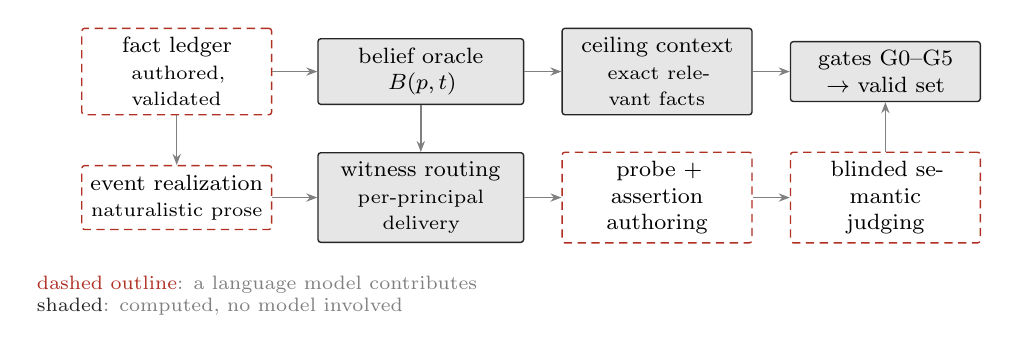
\begin{tikzpicture}[
  node distance=0pt,
  box/.style={draw=ink, line width=.5pt, rounded corners=1pt, align=center,
              font=\footnotesize, minimum height=7.5mm, inner xsep=3pt},
  comp/.style={box, fill=pale!45},
  gen/.style={box, fill=white, draw=accent, densely dashed},
  ar/.style={-{Stealth[length=4pt]}, draw=mid, line width=.5pt},
]
\node[gen,  text width=22mm] (led) at (0,1.5)    {fact ledger\\\scriptsize authored, validated};
\node[comp, text width=24mm] (b)   at (3.1,1.5)  {belief oracle\\$B(p,t)$};
\node[comp, text width=22mm] (ceil)at (6.1,1.5)  {ceiling context\\\scriptsize exact relevant facts};
\node[comp, text width=22mm] (gate)at (9.0,1.5)  {gates G0--G5\\$\rightarrow$ valid set};

\node[gen,  text width=22mm] (ev)  at (0,-0.1)   {event realization\\\scriptsize naturalistic prose};
\node[comp, text width=24mm] (wit) at (3.1,-0.1) {witness routing\\\scriptsize per-principal delivery};
\node[gen,  text width=22mm] (pr)  at (6.1,-0.1) {probe + assertion\\authoring};
\node[gen,  text width=22mm] (jud) at (9.0,-0.1) {blinded semantic\\judging};

\draw[ar] (led) -- (b);
\draw[ar] (b) -- (ceil);
\draw[ar] (ceil) -- (gate);
\draw[ar] (led) -- (ev);
\draw[ar] (ev) -- (wit);
\draw[ar] (wit) -- (pr);
\draw[ar] (pr) -- (jud);
\draw[ar] (jud) -- (gate);
\draw[ar] (b.south) to[out=-90,in=90] (wit.north);

\node[font=\scriptsize, text=mid, align=left, anchor=west] at (-1.9,-1.35)
  {\textcolor{accent}{dashed outline}: a language model contributes\\
   \textcolor{ink}{shaded}: computed, no model involved};
\end{tikzpicture}
\caption{The construction pipeline. The path from the ledger to what is
\emph{true for a principal at a moment} runs entirely through shaded boxes:
$B(p,t)$ is a pure function over the ledger and the event index. Models render
events, author scoring criteria, and judge semantic criteria. No model decides
what is true.}
\label{fig:pipeline}
\end{figure}

\subsection{Ground truth is computed, not asserted}

The design decision everything else rests on is that this benchmark's answer key
is a function, not a list of question--answer pairs written by a model
(Figure~\ref{fig:pipeline}).

Each simulated organization has a private ledger of facts: decisions, working
rules, preferences, commitments, each with a tier (\code{personal}, \code{team},
\code{project}, \code{org}, \code{external}), a capacity
(\code{formal\_decision} $>$ \code{directive} $>$ \code{opinion} $>$
\code{speculation}), a visibility, a validity window, and the events that
evidence it. From the ledger and the event index we compute the \textbf{expected
belief state} $B(p,t)$: every fact that principal is entitled to hold at that
moment. A fact is in $B$ when the principal witnessed it, when its visibility
permits them, when it is valid and unsuperseded at $t$, and when its decay class
still holds. Superseded facts move to a historical set $B_{\mathrm{hist}}$ rather
than vanishing, because a superseded plan must stop driving behavior while
staying retrievable.

Conflicts resolve by stated precedence: higher capacity first; at equal capacity
the tier matching the \emph{artifact} being produced wins, so an org policy
governs an org-facing document and a personal preference governs a personal one;
then recency. A pair that remains tied is not a defect to be broken arbitrarily
but a genuine unresolved contradiction, where correct behavior is surfacing the
conflict rather than silently picking. Rule two is what makes precedence
contextual instead of a fixed hierarchy, and it is the mechanism the scope
archetypes probe.

$B$ is a pure function over (ledger, event index) and is the single scoring
oracle. Two consequences matter for validity. Ambiguity in $B$ is a spec bug that
blocks release rather than a judgement call resolved per item, and both spec bugs
found this way were fixed before any screening: distributed facts originally
required witnessing only one evidence event, which let principals hold facts they
could not have assembled, and departed principals needed an explicit empty belief
state. More importantly, no language model is anywhere in the ground-truth path.
The models render events and author scoring criteria; they never decide what is
true.

\subsection{Streams, witnesses, and what the system under test sees}

Each organization's history is a stream of naturalistic communication: meetings,
DMs, team and org chat, email threads, documents, tickets, pull requests,
calendar entries, with facts embedded in the prose as a person would express
them, in the author's voice, never in ledger-canonical form. Fact annotations are
stripped before the stream reaches a system under test; the annotated copy is
private to scoring.

There is no global feed. The runner delivers each event only to the principals
who witnessed it: participants always, plus anyone entitled to the surface it
appeared on, since channel history is readable. A decision taken in a platform
standup reaches a growth-team principal only if some later event carries it
across, or if the memory layer under test does. That is what makes propagation a
measurable property rather than an assumption, and it is why a system pooling
everything and a system respecting visibility receive different inputs by
construction. The adapter's entire ingestion surface is one call,
\code{ingest(principal\_id, event)}, invoked once per witness per event; what a
system does internally, whether one shared store or per-principal stores, is its
own business, and it is scored against $B(p,t)$.

Realism is a set of generator obligations, not an aspiration. At least 60\% of
event content is operational filler embedding no probed fact, so a memory system
has to find signal rather than summarize everything. Every probed fact is
accompanied by at least two distractor facts, including at least one near-miss
differing by a single attribute: wrong tier, expired, or lower authority. No
fact's canonical text may appear verbatim in more than one event, which forces
paraphrase and blocks string-match shortcuts. Canary strings sit in event text at
low frequency for post-hoc contamination detection. Timelines are sized so the
annotation-stripped transcript exceeds roughly 500k tokens, which keeps
full-transcript-in-context an honest but costly baseline rather than a free win.

Salience parity is achieved by construction and then tested. Distractor type,
register, shape, length, and numeric form mirror the probed mix, and positions
are assigned mechanically to class-stratified band centers rather than by
re-rendering until a lint passes. The test is a blinded discrimination check: a
rater sees 20 excerpts, half embedding probed facts and half distractor-only, and
must not beat 65\%. Machine raters across five seeds scored 58/100 in aggregate
(binomial $p = 0.067$, not significantly above chance); human raters scored 50\%
and 60\% on the two seeds a rater could take uncontaminated. One residual is
documented rather than resolved: seed 3 repeatedly scores above the others
(42/60 across three independent samples, $p \approx 0.001$), two targeted content
passes failed to remove it, and it ships disclosed, with users of
salience-sensitive analyses pointed at the other seeds.

\begin{figure}[t]
\centering
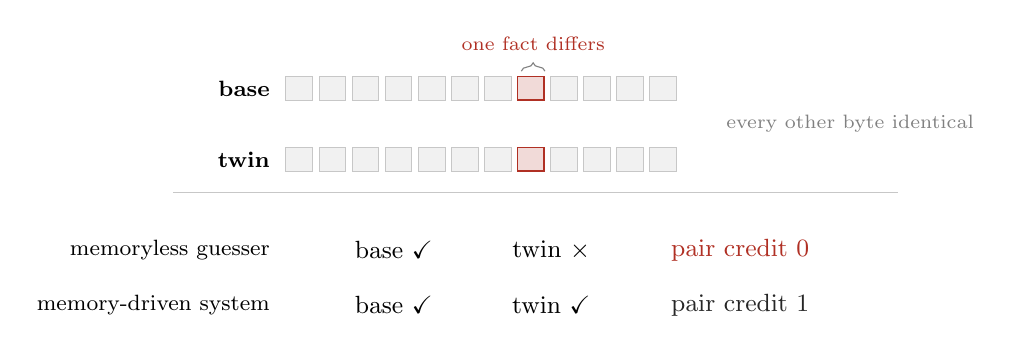
\begin{tikzpicture}[
  font=\footnotesize,
  ev/.style={draw=pale, fill=pale!25, minimum width=3.4mm, minimum height=3mm,
             inner sep=0pt, line width=.3pt},
  delta/.style={draw=accent, fill=accent!18, minimum width=3.4mm,
                minimum height=3mm, inner sep=0pt, line width=.6pt},
]
\node[anchor=east, font=\footnotesize\bfseries] at (-0.25,1.5) {base};
\node[anchor=east, font=\footnotesize\bfseries] at (-0.25,0.6) {twin};
\foreach \i in {0,...,11}{
  \pgfmathsetmacro{\x}{\i*0.42}
  \ifnum\i=7
    \node[delta] at (\x,1.5) {};
    \node[delta] at (\x,0.6) {};
  \else
    \node[ev] at (\x,1.5) {};
    \node[ev] at (\x,0.6) {};
  \fi
}
\draw[decorate, decoration={brace, amplitude=3pt}, draw=mid]
  (2.82,1.72) -- (3.12,1.72);
\node[font=\scriptsize, text=accent, anchor=south] at (2.97,1.86)
  {one fact differs};
\node[font=\scriptsize, text=mid, anchor=west] at (5.3,1.05)
  {every other byte identical};

\draw[draw=pale, line width=.4pt] (-1.6,0.18) -- (7.6,0.18);

\node[anchor=east] at (-0.25,-0.55) {memoryless guesser};
\node[anchor=east] at (-0.25,-1.25) {memory-driven system};
\node[font=\small] at (1.2,-0.55) {base \checkmark};
\node[font=\small] at (3.2,-0.55) {twin $\times$};
\node[font=\small, text=accent] at (5.6,-0.55) {pair credit 0};
\node[font=\small] at (1.2,-1.25) {base \checkmark};
\node[font=\small] at (3.2,-1.25) {twin \checkmark};
\node[font=\small, text=ink] at (5.6,-1.25) {pair credit 1};
\end{tikzpicture}
\caption{Pair credit via counterfactual twins. The twin organization is
regenerated from the same seed with one fact changed and everything else held
byte-identical. A guess that happens to match a model's priors clears the base
side and fails the twin, because the twin's answer is the one those same priors
argue against. Credit is the conjunction, so priors earn nothing.}
\label{fig:twin}
\end{figure}

\subsection{Probes are work, and every probe has a twin}

A probe is not a question. It is a work task issued to a principal's agent at a
point in the timeline: write the announcement, draft the checklist, prepare the
review note. What is scored is whether the resulting artifact behaves as the
organization's knowledge requires. Probes are injected only at evaluation time
and never appear in the ingested stream, which is the countermeasure to tuning a
system on the questions.

Four archetypes instantiate the capability ladder. A4 and A7 sit at rung 1,
alignment, where the right tier must win and current truth must drive behavior;
A1 at rung 2, coordination, where knowledge must cross principals; A2 at rung 3,
compounding, where the organization should apply its own history unprompted.
Rung 0, plain retention, is where existing memory benchmarks live and where long
context saturates; it is implicit in every probe and never headlined. v1 is a
deliberate vertical slice, at least one archetype on every rung above retention,
rather than exhaustive coverage of any one rung.

Every probed fact has a counterfactual variant, and the generator produces a
\textbf{twin organization} from the same seed and the same timeline skeleton with
the delta facts re-rendered (Figure~\ref{fig:twin}). The same probe runs against
both. An instance is credited \textbf{only when both sides pass}: correct
behavior on the base organization, and correctly \emph{different} behavior on the
twin. Passing one side scores zero for the pair.

This is the single most load-bearing design choice in the dataset, because it is
what makes a plausible guess worthless. A fact invented by a language model often
coincides with that model's own prior, whether a naming convention, a review
threshold, or a default cadence, and a memoryless system can guess the base side
at a rate that would flatter it badly. It cannot guess both sides. Section~4.5
reports what this buys: under a memoryless worker, 4 of 125 instances earn pair
credit.

Assertions come in several kinds, among them \code{fact\_applied},
\code{fact\_absent}, \code{scope\_correct} and \code{conflict\_flagged}. Each is
checked by regex, by structural parse, or by a blinded semantic judge. Which
checker is allowed where was settled by measurement rather than preference.
Applied-content assertions written as regexes failed 39--42\% of ceiling runs,
because a deliverable paraphrases around any anchor; absence detectors failed
4\% and semantic criteria 9--17\%. Spec v0.3 therefore requires the semantic
checker for applied content and reserves regex for absence detectors. Assertion
text was model-authored under a fixed prompt and accepted only after mechanical
validation: answer-token hygiene, 4-gram overlap against the task text, and
pattern cross-validation requiring each pattern to match every surface variant of
its own side and no variant of the other side or of a sibling fact. One further
authoring rule came out of failure adjudication and matters more than it looks:
an assertion must never punish content drawn from a different co-valid fact of
the same cluster, because complementary facts are not competing answers.

\subsection{Screening: which items actually measure memory}

Every probe instance runs in three conditions. \code{floor} gives the task alone
with no organizational context. \code{ceiling} gives the task plus exactly the
relevant facts from $B(p,t)$, rendered canonically. \code{sut} gives whatever the
system under test provides. A system's score is normalized as
$(\mathrm{sut} - \mathrm{floor}) / (\mathrm{ceiling} - \mathrm{floor})$.

The floor and ceiling conditions are not only a normalization; they are the
screen. An instance is valid when its ceiling passes, its twin ceiling passes,
and its floor output fails at pair level. A ceiling that fails means the item
measures reasoning rather than memory: the facts were supplied and the worker
still could not produce the artifact. A floor that passes means the item is
answerable without memory at all. Both get dropped, and the per-side floor pass
rate survives as a reported \code{guessability} figure per cluster.

Two revisions to this rule were forced by measurement and are dated before the
evidence they govern. The floor gate moved to pair level once it was clear that
canonical facts sometimes coincide with industry defaults, so a per-side rule
discarded valid pairs for the exact reason the twin design exists. And screening
moved from clusters to instances: requiring all three instances of a cluster to
be valid demands per-run reliability near 98\%, since $0.9^6 \approx 0.53$
cluster survival follows even at 9\% instance noise, which no realistic
worker--judge pair delivers at $n=3$. A cluster now survives with at least 2 of 3
valid instances and ships only those. Both the instance-level and the stricter
all-instances counts are reported throughout.

Semantic verdicts are produced blind. \code{judge-export} writes each output with
its criteria under opaque ids, stripped of probe identity, condition, and
base-versus-twin side; fresh judge agents read only that batch file;
\code{judge-import} validates the ids and criterion keys before anything is
recorded. The judge model is never the worker model and never the family that
authored or repaired the criteria being judged, and the rubric is versioned
verbatim in the repository. Blinding is enforced in code rather than by
instruction. It is worth reporting that blinding changed little: an earlier
unblinded pass over the same seed-1 material agreed with the blinded verdicts on
97.6\% of criteria, 26 flips out of 1{,}092, split 14 True$\rightarrow$False
against 12 False$\rightarrow$True with no systematic direction. Blinding is cheap
insurance here rather than a large correction, and we would rather publish that
null than imply we caught a bias we did not measure.

\subsection{What the released dataset is}

Seeds 1--3, probe-spec v0.4.3, judge rubric v2: \textbf{371 valid paired
instances} (A1 50, A2 43, A4 106, A7 172). Per seed the valid-instance counts are
125/131/115, from cluster survival of 46/54, 46/54, 40/54; the stricter
all-instances counts are 33, 39 and 35. Construction produced 54 clusters
$\times$ 3 instances $\times$ 5 organizations, 810 instances in total, of which
seeds 4 and 5 are withheld unscreened as holdouts.

\textbf{All three instance gates fail.} The prespecified threshold was 135 valid
instances per seed, and the three seeds delivered 125, 131, and 115.
\textbf{Seed 3's cluster gate also fails}, at 40 surviving clusters against a
floor of 45. No probe that failed a gate was repaired, no criterion was rewritten
to recover an instance, and no gate was relaxed after it bound. The shortfall is
structured rather than random: it is the residual tail of counterfactual-anchoring
failure on the twin side, the same defect family that drives cluster drops, and
the prespecified v2 response is to over-generate four instances per cluster and
require counterfactuals to invert the aspect the task actually elicits.

The dataset was frozen on 2026-08-15 before any system was evaluated, and the
freeze is corroborated by dated commits rather than by assertion.

\subsection{Worker and harness pinning}

All screening ran under a single pinned worker: gpt-5.4 at medium reasoning
effort behind codex-cli 0.144.5, with the binary pin enforced in code rather than
by convention, because the system \code{codex} upgrades silently. The pin is not
housekeeping. Section~4.2 shows that which items survive screening is a property
of the worker, \S4.3 shows that the agent harness around identical weights
changes outcomes enough to fail a prespecified equivalence bar, and \S4.6 reports
what happened when the provider withdrew the pinned model mid-study.

\section{Validity study: the results core}

Every number below was already measured; none of it needed the deprecated worker.

\begin{figure}[t]
\centering
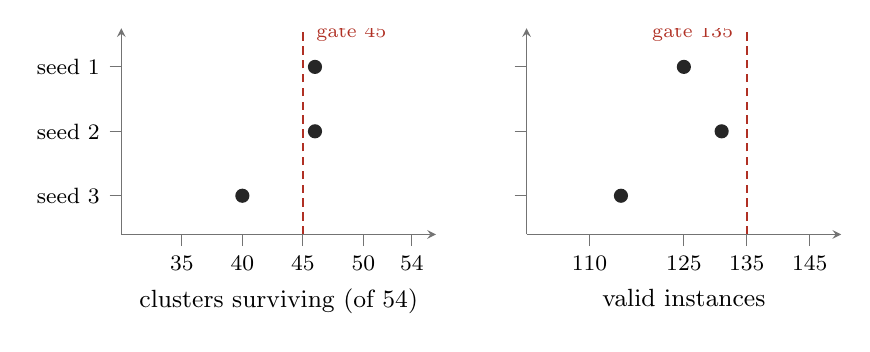
\begin{tikzpicture}
\begin{axis}[
  tufte, width=.46\textwidth, height=4.2cm,
  xmin=30, xmax=56, ymin=0.4, ymax=3.6,
  ytick={1,2,3}, yticklabels={seed 3, seed 2, seed 1},
  xlabel={clusters surviving (of 54)},
  xtick={35,40,45,50,54},
  scatter/use mapped color={draw=ink, fill=ink},
  name=left,
]
\addplot[only marks, mark=*, mark size=2.1pt, draw=ink, fill=ink]
  coordinates {(40,1) (46,2) (46,3)};
\draw[draw=accent, line width=.6pt, densely dashed]
  (axis cs:45,0.4) -- (axis cs:45,3.6);
\node[font=\scriptsize, text=accent, anchor=south west] at
  (axis cs:45.3,3.25) {gate 45};
\end{axis}

\begin{axis}[
  tufte, width=.46\textwidth, height=4.2cm,
  at={(left.south east)}, xshift=1.15cm, anchor=south west,
  xmin=100, xmax=150, ymin=0.4, ymax=3.6,
  ytick={1,2,3}, yticklabels={,,},
  xlabel={valid instances},
  xtick={110,125,135,145},
]
\addplot[only marks, mark=*, mark size=2.1pt, draw=ink, fill=ink]
  coordinates {(115,1) (131,2) (125,3)};
\draw[draw=accent, line width=.6pt, densely dashed]
  (axis cs:135,0.4) -- (axis cs:135,3.6);
\node[font=\scriptsize, text=accent, anchor=south east] at
  (axis cs:134.4,3.25) {gate 135};
\end{axis}
\end{tikzpicture}
\caption{Gate G3 by seed. Every point left of a dashed rule is a failure carried
into the release rather than repaired. All three instance gates fail; seed 3's
cluster gate fails as well. Nothing was topped up to cross a line.}
\label{fig:gates}
\end{figure}

\subsection{Gate results}

Six gates run during construction, and their outcomes are reported as measured.
G0 and G1, the belief-oracle test suite and the schema, oracle cross-check,
ambiguity scan, and interleaving checks, passed on every seed. G2's machine side
passed: structural regeneration, realization checks, and the release-blocking
stream lint covering marker round-trip, visibility consistency, salience
permutation tests, a noise floor, and canaries all report green across five
organizations and their twins. Two of G2's human items remain open by the freeze,
and the salience residual on seed 3 is documented rather than repaired (\S3.2).

G3 is where the failures are (Figure~\ref{fig:gates}), and they are the reason
the rest of this section is worth reading.

\begin{table}[h]
\centering\small
\begin{tabular}{lccll}
\toprule
seed & clusters surviving & valid instances & instance gate ($\geq$135) & cluster gate ($\geq$45)\\
\midrule
1 & 46/54 & 125 & \textbf{FAIL} & pass\\
2 & 46/54 & 131 & \textbf{FAIL} & pass\\
3 & 40/54 & 115 & \textbf{FAIL} & \textbf{FAIL}\\
\bottomrule
\end{tabular}
\end{table}

Two further prespecified bars failed: the harness-equivalence study of \S4.3, and
G4 in \S4.4. Four failures against one clean positive result, the memoryless
floor of \S4.5.

No probe that failed a gate was repaired to recover it, no criterion was
rewritten after seeing that it cost an instance, and no threshold moved once it
bound. Where repairs did happen they were made blind to direction, before the
evidence they touched, and are recorded with the risk stated in advance: the
cross-organization lineage sweep was applied without knowing whether it would
move counts up or down, and it moved them both ways. The consistency pass found
exactly two defects across five seeds, single filler lines asserting rule content
that contradicted a probed fact, and both were replaced with inert material.

A gate that is relaxed once it binds was never a gate, so we would rather publish
a dataset that fails its own thresholds than one whose thresholds were chosen
after the fact. That is the whole argument for trusting the numbers that did
pass.

\subsection{Probe validity is task-model-relative}

Screening asks whether a worker given exactly the right facts can produce the
artifact the task requires. That question has a different answer for different
workers, and the size of the difference is the finding.

Under identical strict rules, \textbf{37 of 54} probe clusters survived the
ceiling gate for gpt-5.4 and \textbf{17 of 54} for gpt-5.4-mini, a smaller model
from the same family. Less than half. Nothing about the probes changed between
those two numbers; the items are the same items and the rule is the same rule.

The consequence is that a valid item is not a property of the item. It is a
property of the pair, item and worker, and a released valid set is defined
relative to the model that screened it. This is not a quirk of our design. Any
benchmark that decides which of its items are answerable by checking whether a
model can answer them inherits the same relativity, whether or not it says so.
Most do not say so, and many do not fix the worker at all, which makes their item
sets quietly unreproducible.

We handle it by pinning the worker, reporting the pin everywhere a number
appears, and publishing the per-worker re-screening procedure so a future user
can re-derive a valid set under whatever model they have. Section~4.6 is what
happens when that future arrives sooner than expected.

\begin{figure}[t]
\centering
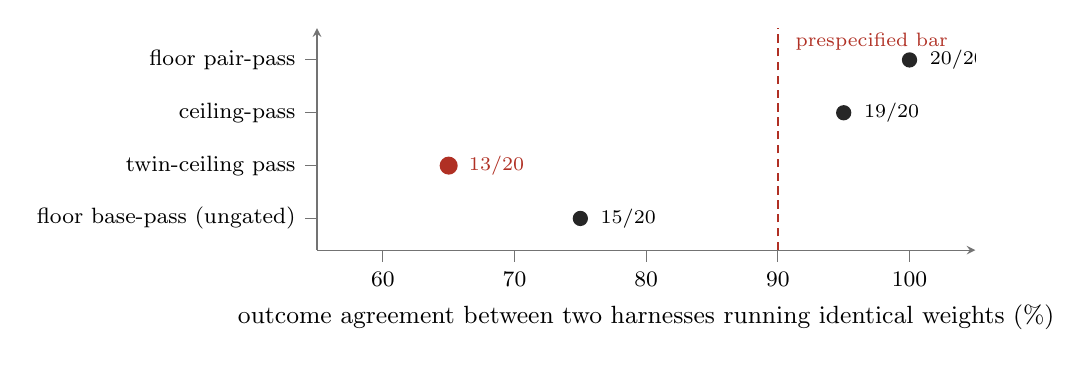
\begin{tikzpicture}
\begin{axis}[
  tufte, width=.82\textwidth, height=4.4cm,
  xmin=55, xmax=105, ymin=0.4, ymax=4.6,
  ytick={1,2,3,4},
  yticklabels={floor base-pass (ungated), twin-ceiling pass, ceiling-pass, floor pair-pass},
  xlabel={outcome agreement between two harnesses running identical weights (\%)},
  xtick={60,70,80,90,100},
  yticklabel style={font=\footnotesize},
]
\draw[draw=accent, line width=.7pt, densely dashed]
  (axis cs:90,0.4) -- (axis cs:90,4.6);
\node[font=\scriptsize, text=accent, anchor=west] at (axis cs:90.6,4.35)
  {prespecified bar};
\addplot[only marks, mark=*, mark size=2.3pt, draw=ink, fill=ink]
  coordinates {(75,1) (95,3) (100,4)};
\addplot[only marks, mark=*, mark size=2.8pt, draw=accent, fill=accent]
  coordinates {(65,2)};
\node[font=\scriptsize, anchor=west] at (axis cs:100.8,4) {20/20};
\node[font=\scriptsize, anchor=west] at (axis cs:95.8,3) {19/20};
\node[font=\scriptsize, anchor=west, text=accent] at (axis cs:65.8,2) {13/20};
\node[font=\scriptsize, anchor=west] at (axis cs:75.8,1) {15/20};
\end{axis}
\end{tikzpicture}
\caption{Harness sensitivity. Sixty runs, 20 per condition, identical gpt-5.4
weights, identical prompts, identical blinded scoring; only the agent scaffold
differs. Agreement is near-total where the task is easy to fail or easy to pass,
and collapses in the one condition that is hard to satisfy. The study failed its
own acceptance rule, so the second harness was confined to non-protocol work.}
\label{fig:harness}
\end{figure}

\subsection{Harness sensitivity}

Before admitting a second agent harness to any protocol path we ran a
prespecified equivalence study: 60 seed-1 runs, 20 per condition, RNG seed fixed,
scored through the identical blinded pipeline, with the acceptance rule written
down before any run. The bar was outcome agreement $\geq 90\%$ per condition. The
two harnesses ran identical gpt-5.4 weights at identical effort; only the agent
scaffold differed.

The study failed its own acceptance rule (Figure~\ref{fig:harness}), and the
second harness was confined to QA and non-protocol work on that evidence. Two
things are worth drawing out.

The disagreement is not uniform: it concentrates in the conditions that are
hardest to satisfy. Where the task is easy to fail (the memoryless floor, at
100\%) or easy to pass (the ceiling with facts injected, at 95\%) the harnesses
agree. The twin ceiling asks a worker to produce a deliverable consistent with a
counterfactual fact while an almost identical base fact is absent, and there the
same weights behind different scaffolds disagree on more than a third of
outcomes.

The consequence for the field is the one worth carrying: the harness is part of
the consumer, not a neutral pipe to the weights. A benchmark that pins a model and
not its harness has not pinned its worker, and a result reported without a harness
version is unanchored. It also explains why re-anchoring (\S4.6) has to fix the
harness version alongside the model.

\subsection{Judge validation}

We ran two checks on the judge: a cheap automated one and an expensive human one.
They disagree about whether the judge is sound, and the reason they disagree is
the most transferable result in this paper.

\subsubsection*{The 20-decoy false-accept audit: PASS, and blind to the defect}

Deliberately wrong-but-topical outputs were judged blind against the real
criteria: \textbf{2/41 false accepts as measured, 0/39 after adjudicating two
criteria an under-specified decoy legitimately satisfied}. Read on its own this
says the judge does not accept plausible-sounding wrong answers, which is the
LoCoMo failure mode of \S2.3.

Resolving those 41 criteria back to their kinds shows why that reading was
premature: \textbf{30 were \code{fact\_applied}, 11 were \code{scope\_correct},
and none were \code{fact\_absent}}. A decoy is built by stating wrong values, so
it exercises criteria that demand content. A criterion phrased as absence is
satisfied by an output that never raises the topic, so a decoy cannot probe it
without being built differently. The audit was structurally incapable of
detecting a failure on absence criteria, and that is exactly where the failure
turned out to be.

\subsubsection*{G4 judge--human agreement: measured 2026-09-14, FAIL}

The blinded 150-pair packet was rated by the single author-rater (the disclosed
downgrade, \S7 item 2) and scored against the committed judge verdicts.

\begin{table}[h]
\centering\small
\begin{tabular}{lccc}
\toprule
 & $n$ & raw agreement & $\kappa$\\
\midrule
\textbf{overall} & 150 & 0.813 & \textbf{0.537} (gate $\kappa \geq 0.75$: FAIL)\\
\code{fact\_applied} & 72 & 0.819 & 0.605\\
\code{scope\_correct} & 34 & 0.794 & 0.561\\
\code{fact\_absent} & 44 & 0.818 & \textbf{0.166}\\
\bottomrule
\end{tabular}
\end{table}

\begin{figure}[t]
\centering
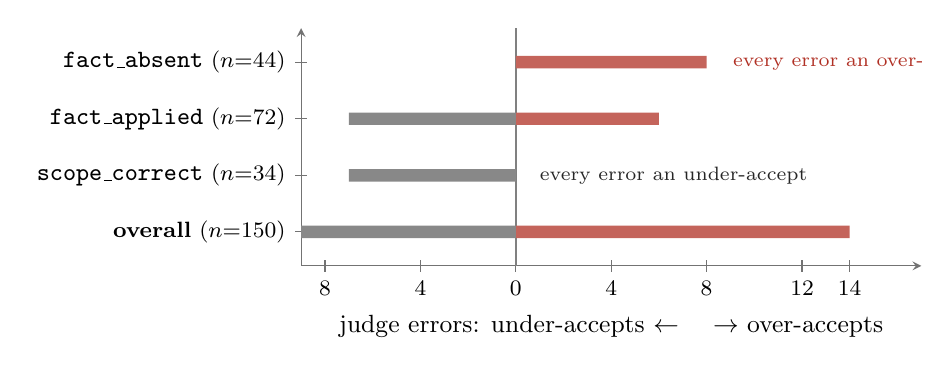
\begin{tikzpicture}
\begin{axis}[
  tufte, width=.78\textwidth, height=4.6cm,
  bar width=4.5pt,
  xmin=-9, xmax=17, ymin=0.4, ymax=4.6,
  ytick={1,2,3,4},
  yticklabels={\textbf{overall} ($n{=}150$), \code{scope\_correct} ($n{=}34$),
               \code{fact\_applied} ($n{=}72$), \code{fact\_absent} ($n{=}44$)},
  yticklabel style={font=\footnotesize},
  xlabel={judge errors: under-accepts $\leftarrow$ \quad $\rightarrow$ over-accepts},
  xtick={-8,-4,0,4,8,12,14},
  xticklabels={8,4,0,4,8,12,14},
  axis lines=left,
]
\draw[draw=mid, line width=.5pt] (axis cs:0,0.4) -- (axis cs:0,4.6);
\addplot[xbar, draw=none, fill=accent!75]
  coordinates {(8,4) (6,3) (0,2) (14,1)};
\addplot[xbar, draw=none, fill=ink!55]
  coordinates {(0,4) (-7,3) (-7,2) (-14,1)};
\node[font=\scriptsize, text=accent, anchor=west] at (axis cs:8.7,4)
  {every error an over-accept};
\node[font=\scriptsize, text=ink, anchor=west] at (axis cs:0.6,2)
  {every error an under-accept};
\end{axis}
\end{tikzpicture}
\caption{The symmetry is a cancellation, not a property. On absence-phrased
criteria every judge error is an over-accept; on scope criteria every error is an
under-accept. They cancel to 14 against 14 in aggregate, and the bias index is
exactly 0.000, purely because this packet happens to contain 44 of the first kind
and 34 of the second. A different mix of criterion kinds would not cancel.}
\label{fig:cancellation}
\end{figure}

Three things about this failure are worth stating precisely, because the headline
number alone misleads in both directions.

\textbf{The symmetry is a cancellation, not a property.} Aggregate disagreement
splits 14 and 14, and both raters label 72.0\% of items positive, which invites
the conclusion that the judge is unbiased noise. The per-kind confusion matrix
says otherwise (Figure~\ref{fig:cancellation}): on \code{fact\_absent} the judge
over-accepts on all 8 of its errors, on \code{scope\_correct} it under-accepts on
all 7, and \code{fact\_applied} is genuinely mixed at 7 and 6. Any system scored
on this benchmark inherits a bias whose sign depends on which archetypes its
instances draw from, which is a property of the judge that no single agreement
number reveals.

\textbf{The judge barely discriminates on absence criteria.} It returns
\textsc{false} on 1 of 44 absence-phrased items; the human rater returns
\textsc{false} on 9. A criterion of the form ``does not present X as current''
is, in this judge's hands, close to automatically satisfied.

\textbf{$\kappa = 0.166$ on \code{fact\_absent} is a base-rate artifact} and must
not be read as ``absence criteria are harder to agree on''. Raw agreement on that
kind is 0.818, statistically indistinguishable from \code{fact\_applied} at 0.819
and \code{scope\_correct} at 0.794. $\kappa$ collapses only because the judge's
97.7\% positive rate pushes chance agreement to 0.782, leaving almost no
headroom. We state this explicitly because the opposite reading is the natural
one and we made it ourselves in an earlier draft.

\textbf{On the gate itself.} The gate was $\kappa \geq 0.75$. It failed at 0.537.
That stands, and the diagnostics below explain the mechanism rather than soften
the verdict. They were computed after the result and are labelled post-hoc; none
was prespecified.

\begin{table}[h]
\centering\small
\begin{tabular}{lcccccc}
\toprule
 & agreement & $\kappa$ & prevalence idx & bias idx & PABAK & Gwet AC1\\
\midrule
\code{fact\_absent} & 0.818 & 0.166 & \textbf{0.773} & 0.182 & 0.636 & 0.772\\
\code{fact\_applied} & 0.819 & 0.605 & 0.292 & 0.014 & 0.639 & 0.667\\
\code{scope\_correct} & 0.794 & 0.561 & 0.324 & 0.206 & 0.588 & 0.627\\
\textbf{overall} & 0.813 & \textbf{0.537} & 0.440 & \textbf{0.000} & 0.627 & 0.687\\
\bottomrule
\end{tabular}
\end{table}

This is the kappa paradox: when one label dominates, $\kappa$ penalizes residual
disagreement disproportionately. Prevalence-adjusted statistics put the same data
between 0.59 and 0.77, so the disagreement is not the near-chance concordance a
bare $\kappa = 0.537$ suggests. And we prespecified $\kappa$ rather than raw
agreement precisely so an unbalanced task could not be dressed up as validity,
which means we do not now get to discover the objection to our own gate on the
day it fails. Leading with AC1 $= 0.687$ and putting $\kappa$ in a footnote would
be the spin version of this paragraph, and a reader who knows the reliability
literature would recognize the move immediately.

The bias index is worth reading alongside the confusion matrix. Overall it is
\textbf{0.000}, a perfectly unbiased judge by that measure, while within kinds it
is 0.182 and 0.206 pointing in opposite directions. The aggregate figure is not
evidence of an unbiased judge; it is the numerical signature of two biases
cancelling, and it is the clearest demonstration that per-kind reporting is not
optional.

\subsubsection*{Where the leniency lands}

\textbf{The over-accepts concentrate on the counterfactual side.} Of the judge's
14 over-accepts, 11 fall on twin-side criteria against 3 on base-side; its
under-accepts split evenly, 7 and 7. This follows from the design: a twin asserts
that the base fact is \emph{not} presented, so absence-phrased criteria live
disproportionately on that side (26 of the 44 sampled absence items). Pair credit
requires both sides to pass, so a judge that waves twin sides through inflates
instance credit directly. The error is in the direction that flatters a system
under test.

\textbf{The exposed fraction of the dataset is not small.} 218 of the 371 valid
instances (58.8\%) carry at least one \code{fact\_absent} criterion: 199 on the
base side, 207 on the twin side, 188 on both.

Why the class behaves this way is mechanical rather than mysterious. ``The note
does not present the 48h SLA as current'' is satisfied by a note that never
mentions the SLA at all, so silence passes. The class has a degenerate pass mode,
the judge sits at 97.7\% positive because of it, and $\kappa$ has almost no
variance to track. This is therefore as much a criterion-design defect as a judge
defect: an absence criterion carries little discriminative signal unless it is
paired with a positive criterion demanding the replacement value.

\begin{figure}[t]
\centering
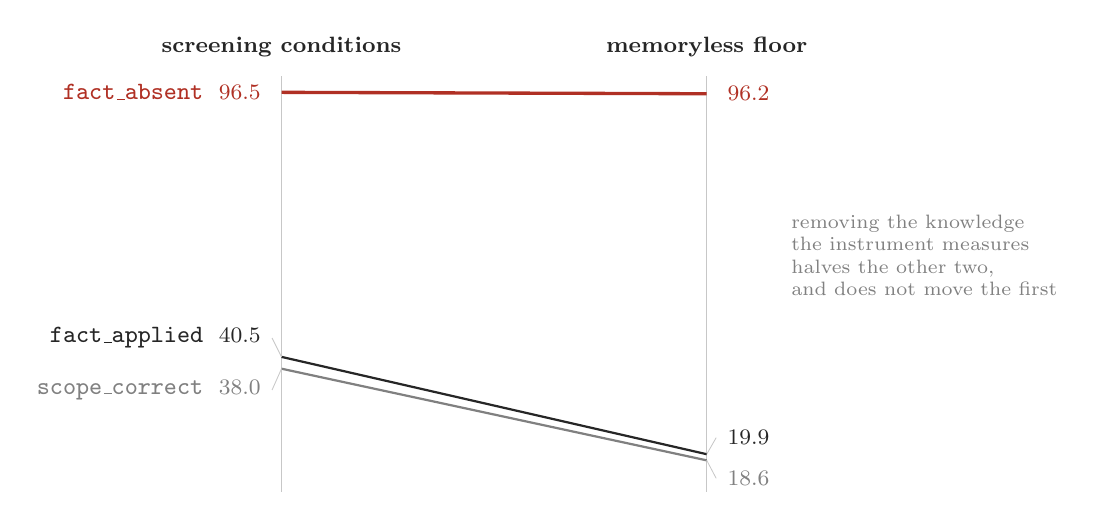
\begin{tikzpicture}[font=\footnotesize]
\def\xa{0}
\def\xb{5.4}
% 1 percentage point = 0.06cm. Line endpoints sit at their true values; only
% the two crowded TEXT labels are nudged, each with a leader line back to its
% endpoint, so the geometry still reads at lie factor 1.
\newcommand{\yy}[1]{#1*0.06}

\draw[draw=pale, line width=.4pt] (\xa,\yy{12}) -- (\xa,\yy{100});
\draw[draw=pale, line width=.4pt] (\xb,\yy{12}) -- (\xb,\yy{100});
\node[anchor=south, font=\footnotesize\bfseries, text=ink] at (\xa,\yy{102})
  {screening conditions};
\node[anchor=south, font=\footnotesize\bfseries, text=ink] at (\xb,\yy{102})
  {memoryless floor};

% fact_absent: flat, and it is the point of the figure
\draw[draw=accent, line width=1.2pt] (\xa,\yy{96.5}) -- (\xb,\yy{96.2});
\node[anchor=east, text=accent] at (\xa-0.14,\yy{96.5})
  {\code{fact\_absent}\ \ 96.5};
\node[anchor=west, text=accent] at (\xb+0.14,\yy{96.2}) {96.2};

% fact_applied: halves. Label nudged up, leader back to the true endpoint.
\draw[draw=ink, line width=.8pt] (\xa,\yy{40.5}) -- (\xb,\yy{19.9});
\draw[draw=pale, line width=.3pt] (\xa-0.12,\yy{44.5}) -- (\xa,\yy{40.5});
\draw[draw=pale, line width=.3pt] (\xb,\yy{19.9}) -- (\xb+0.12,\yy{23.4});
\node[anchor=east, text=ink] at (\xa-0.14,\yy{44.5})
  {\code{fact\_applied}\ \ 40.5};
\node[anchor=west, text=ink] at (\xb+0.14,\yy{23.4}) {19.9};

% scope_correct: halves. Label nudged down, leader back to the true endpoint.
\draw[draw=mid, line width=.8pt] (\xa,\yy{38.0}) -- (\xb,\yy{18.6});
\draw[draw=pale, line width=.3pt] (\xa-0.12,\yy{33.5}) -- (\xa,\yy{38.0});
\draw[draw=pale, line width=.3pt] (\xb,\yy{18.6}) -- (\xb+0.12,\yy{14.8});
\node[anchor=east, text=mid] at (\xa-0.14,\yy{33.5})
  {\code{scope\_correct}\ \ 38.0};
\node[anchor=west, text=mid] at (\xb+0.14,\yy{14.8}) {18.6};

\node[anchor=west, font=\scriptsize, text=mid, align=left]
  at (\xb+0.95,\yy{62}) {removing the knowledge\\the instrument measures\\halves the other two,\\and does not move the first};
\end{tikzpicture}
\caption{Judge positive rate per criterion kind (\%), screening conditions
against the memoryless floor. Under a worker with no organizational context,
\code{fact\_applied} and \code{scope\_correct} roughly halve, which is what a
discriminating criterion does. \code{fact\_absent} does not move. Measured on all
5{,}398 committed rubric-v2 verdicts, with no human labels involved.}
\label{fig:slopegraph}
\end{figure}

\subsubsection*{The mechanism at corpus scale, without human labels}

Everything above rests on 44 absence-phrased items in one 150-pair packet, which
is a thin base for a claim about the instrument as a whole. The mechanism, a
criterion class with a degenerate pass mode, can be measured without human labels
at all, on every verdict the project has committed, and it was.

Joining all \textbf{5{,}398} committed rubric-v2 criterion verdicts to their
assertion kind gives the judge's positive rate per class (the join is
deterministic and lossless): \code{fact\_absent} \textbf{96.4\%} ($n = 1{,}463$),
\code{fact\_applied} 39.0\% ($n = 2{,}677$), \code{scope\_correct} 36.9\% ($n =
1{,}258$). The 97.7\% observed on 44 sampled items was not a sampling artifact.
The rate holds across all five sources of verdicts with no exception, from 93.2\%
to 98.9\%.

The memoryless floor run supplies the control that makes this diagnostic rather
than merely descriptive (Figure~\ref{fig:slopegraph}). Under a worker that
demonstrably cannot know the facts, \code{fact\_applied} collapses to 19.9\% and
\code{scope\_correct} to 18.6\%. \code{fact\_absent} holds at \textbf{96.2\%},
statistically unmoved. A criterion class that does not respond to removing the
very knowledge the instrument is built to measure is not discriminating; it is
passing by construction, and the two criterion kinds beside it in the same runs,
judged by the same judge under the same rubric, show what responding looks like.

This is a re-analysis of already-committed verdicts rather than a new
measurement: no output was re-run, no criterion re-judged, and no valid set
moved. It was prespecified and dated before it was computed, and it is reported
as a statement about the mechanism, never about accuracy.

\subsubsection*{What the defect does not reach}

The leniency is contained by a structural property of the probe set, which we
checked rather than assumed: \textbf{no side of any instance is scored on absence
criteria alone.} Every base side and every twin side across all 371 valid
instances pairs its absence criteria with at least one criterion demanding
positive content. An output that stays silent, or that knows nothing, cannot pass
even one side on the judge's leniency.

The floor run bears this out empirically. Under a memoryless worker, 4 of 125
instances earned pair credit, which is the result reported in \S4.5. If twin-side
leniency were letting ignorance through, the floor would be visibly above zero,
and it is not. \textbf{The judge defect therefore does not explain away this
paper's one positive result.}

What it does affect is the size of any future number on absence-heavy archetypes.
Exposure is uneven: A4 70.8\% of valid instances, A7 57.0\%, A2 55.8\%, A1
42.0\%. Any score later computed on A4 in particular should be read as an upper
bound rather than an estimate.

\subsubsection*{Why we did not fix it, and why fixing it would not have passed}

Recomputing $\kappa$ on the same 150 pairs with the identified defect removed is
assumption-free, because it only requires flipping verdicts we already have:
as measured, 0.813 / $\kappa$ 0.537, FAIL; every absence false-accept eliminated,
0.867 / 0.688, still FAIL; every false-accept of any kind eliminated, 0.907 /
0.790, PASS; both directional biases eliminated, 0.913 / 0.787, PASS.

\textbf{Repairing the defect we found, perfectly, still fails the gate.} After
removing all 8 absence false-accepts, the residual error is 6 false-accepts and 7
false-rejects on \code{fact\_applied}, which is genuine symmetric noise, plus 7
false-rejects and zero false-accepts on \code{scope\_correct}, where the judge is
already too strict. The two faults point in opposite directions, and rubric
strictness is one dial. Passing requires fixing both biases in opposite
directions and lands at 0.787, a hair over the line and assuming a precision no
rubric edit delivers.

\textbf{The principle.} Even if the arithmetic worked, the criteria were frozen
before this evidence existed, and rewriting them now is the practice \S2.3
condemns: LoCoMo's ground truth and the Mem0/Zep dispute are both the measuring
instrument moving after the measurement. There is a subtler trap too: our 150
human labels are judge-independent, so a new rubric genuinely could be re-scored
against them, but iterating rubric versions until $\kappa$ clears 0.75 stops
measuring judge quality and starts measuring how many attempts were taken. An
unbiased re-measurement needs a held-out calibration set we do not have.

The prespecified v2 fix: pair every absence criterion with a positive criterion
demanding the replacement value, so the class stops having a degenerate pass
mode.

One honest limit on the diagnosis, now narrower than it was. The two halves of
the claim rest on different evidence. That the class has a \textbf{degenerate
pass mode} is demonstrated without human labels, on 1{,}463 verdicts, with the
floor run as a control. That the judge's permissiveness is \textbf{wrong on
particular items} still rests on one rater, and with one rater we cannot separate
judge error from rater error. A second independent rater would settle the second
half and would not change the first.

\subsubsection*{Per-criterion drops: a prespecified rule we measured and declined}

28 criteria fall below the 0.7 raw-agreement threshold. The prespecified rule is
to drop them and disclose the count, never to rewrite them. We report this at
length because the sequence matters more than the outcome.

We committed to applying the rule and recorded that commitment, with the
direction of the change stated as unknown, before any re-score ran. We then ran
it. Dropping the 28 takes the dataset from \textbf{371 to 341 valid instances}
and moves seeds 1 and 2 from a passing cluster gate to a failing one, 46/54
becoming 40/54 and 41/54. Before the drop, three of six gates failed. After it,
all six do. Seed 3 is unchanged, which is the control behaving: none of the 28
criteria are in it.

Having seen that, we kept the frozen 371 and publish the drop as a sensitivity.

The substantive reason stands on its own and predates the result: 25 of the 28
rest on a single sampled judgment and 3 on two, so ``below 0.7'' means one rater
disagreed once, which the tooling itself flags as too weak a basis for dropping
an individual criterion. The objection also stands, and a reader is entitled to
weigh it: we are declining a prespecified rule on the day it bound, after seeing
that applying it would have cost two gate passes. We record both the commitment
and the reversal with dates rather than presenting the decision as though the
number had never been computed.

One gap in the rule needed filling. For 30 instances, dropping removes every
criterion on a scored side, and a side with no criteria passes vacuously. We mark
those unscorable and therefore invalid, which is the strict reading and accounts
for the entire 30-instance difference; a permissive reading would leave the total
near 371. The prespecified rule does not cover the case, so this is our judgement
call and is reported as one.

\subsubsection*{The methodological point, which generalizes past this benchmark}

Two judge-validity checks, run on the same judge under the same rubric, returned
opposite verdicts. The cheap automated one passed and could not have failed,
because decoys are built by stating wrong values and therefore exercise only
criteria that demand content. The expensive human one failed and localized a
specific degenerate class. Anyone building a benchmark judged by a language model
should report judge agreement \textbf{per criterion type}: an aggregate
false-accept rate, and even an aggregate over/under-accept balance, can conceal
opposite directional failures that cancel.

\begin{figure}[t]
\centering
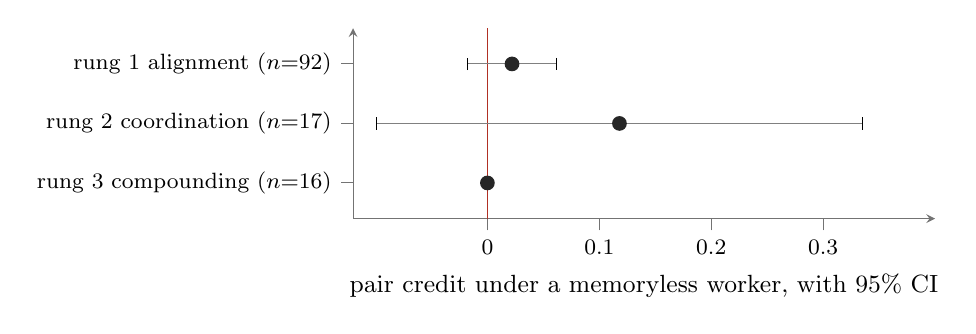
\begin{tikzpicture}
\begin{axis}[
  tufte, width=.74\textwidth, height=4.0cm,
  xmin=-0.12, xmax=0.40, ymin=0.4, ymax=3.6,
  ytick={1,2,3},
  yticklabels={rung 3 compounding ($n{=}16$), rung 2 coordination ($n{=}17$),
               rung 1 alignment ($n{=}92$)},
  yticklabel style={font=\footnotesize},
  xlabel={pair credit under a memoryless worker, with 95\% CI},
  xtick={0,0.1,0.2,0.3},
]
\draw[draw=accent, line width=.6pt] (axis cs:0,0.4) -- (axis cs:0,3.6);
\addplot[only marks, mark=*, mark size=2.2pt, draw=ink, fill=ink,
         error bars/.cd, x dir=both, x explicit, error bar style={draw=mid}]
  coordinates {
    (0.000,1) +- (0,0)
    (0.118,2) +- (0.217,0)
    (0.022,3) +- (0.040,0)
  };
\end{axis}
\end{tikzpicture}
\caption{Floor validation. A worker with no organizational context earns pair
credit on 4 of 125 instances, and every interval includes zero. Rungs 2 and 3
rest on 17 and 16 instances, so the intervals are wide and shown as such.}
\label{fig:floor}
\end{figure}

\subsection{Floor validation: pair credit filters priors}

This is the paper's one clean positive result, and it tests the claim the whole
design rests on: that the instrument measures memory rather than competence.

The memoryless condition ran end to end through the full evaluation pipeline on
seed 1, not as a special case. A worker with no organizational context received
each of the 125 valid instances on both the base and twin sides, and the 250
resulting deliverables were judged blind through the same export and import path
as everything else.

Pair credit came out near zero on every capability rung
(Figure~\ref{fig:floor}): \textbf{rung 1 pair credit 0.022} (95\% CI $\pm$0.040,
$n=92$) for alignment, \textbf{rung 2 0.118} ($\pm$0.217, $n=17$) for
coordination, and \textbf{rung 3 0.000} ($n=16$) for compounding. Four instances
out of 125 earned credit in total, and every interval includes zero.

The mechanism is the twin. A memoryless worker can guess a base side at a rate
well above zero, because a generated fact often matches the priors of a competent
model, and a benchmark crediting single sides would read that as memory.
Requiring the twin side as well removes it, because the twin's answer is the one
those same priors argue against. The design predicted this and the floor measures
it.

Two honest qualifications. Rung 2 rests on 17 instances and rung 3 on 16, so the
intervals are wide and the rung-level claim is weak even though the direction is
not. And this is one seed, because the deprecation stopped the other two before
they ran.

\subsection{Benchmark durability: the deprecation event and re-anchoring}

The dataset was frozen on 2026-08-15. Pilot runs began 2026-09-02. On 2026-09-04
the runs stalled, and what the logs recorded was not an announcement but a wall
of identical worker failures. By the time it was diagnosed the provider had
removed gpt-5.4 from every billing path available to this project, returning a
hard error. The pinned worker had ceased to exist, roughly seven weeks after
being pinned.

Section~4.2 makes the consequence unavoidable. Screening anchors are properties
of a worker. If the worker is gone, the anchors cannot be reproduced, the partial
rows already collected cannot be completed, and rows collected under a successor
cannot be mixed with rows collected under the dead one. Attaching new results to
old anchors would break both the normalization and the pair-validity argument at
once.

The decay literature of \S2.4 treats the data as the perishable component and
answers it with regeneration and refresh. For an agentic benchmark the data is
the durable part. The worker used to establish which items are answerable is the
perishable part, and it perishes on the provider's schedule rather than on the
benchmark's. We have not seen this addressed, and we would not have written it up
as a contribution if it had not happened to us.

The release therefore ships a maintenance contract rather than an assurance. If a
successor worker is pinned, the rule is the nearest same-provider successor at the
time of deprecation; anchors are re-screened for the released seeds under the
frozen gate rules with task text held byte-identical, which is what keeps the
comparison a re-anchoring rather than a new dataset; the result is a new valid set
under the new worker, reported as such; and only then can systems be evaluated.
Anchors and system rows from different workers are never mixed. The procedure is
specified whether or not we ever run it, because a dataset whose validity cannot
be re-established outlives nothing.

\section{The instrument as released}

The dataset ships with the harness that runs it, because a benchmark whose
evaluation code is a description rather than an artifact cannot be reproduced.

\textbf{The adapter surface is deliberately tiny.} A system under test implements
three things: a counters dictionary, \code{ingest(principal, event)}, and
\code{run\_task(principal, task) -> str}. Memory internals are never inspected.
What a system stores, how it indexes, when it consolidates: none of it is
observed or scored, only the behavior of the artifact its worker produces.

Witness routing lives in the runner rather than in any adapter, which keeps
per-principal delivery identical across systems. Participants always witness an
event; org-public events reach every active principal, honouring join and leave
dates; team-confidential events reach team members as of that stream position;
private events reach participants only. Any other visibility value raises rather
than defaulting. A worker failure is recorded as a null deliverable carrying its
error, never as a dropped run, so a system cannot improve its score by failing.

\textbf{Eleven system configurations are registered; ten are runnable in v1.}
Four baselines, namely the memoryless floor, full-transcript long context, a
filesystem-and-grep agent and embedding RAG, plus a lexical BM25 ablation of the
RAG baseline, four market systems selected by published inclusion criteria, and a
per-principal silo ablation of one market system. The eleventh, a typed-memory
reference implementation, is registered and constructible but deferred by the v1
freeze and never run. The grep baseline is there on principle: a memory product
should have to beat a directory of files and a search command.

\textbf{Configurations were frozen before any live run and amended only
mechanically.} The per-system config file was committed 2026-08-27, before any
system was contacted, and states that the only permitted post-smoke changes are
availability fixes, meaning auth flags, timeouts and API-shape corrections,
recorded as dated amendments, never retrieval-quality tuning. Four amendments
followed on 2026-09-02, all dated in git.

Two of those four deserve to be named rather than folded into a summary, because
a reader could reasonably contest whether they are purely mechanical. One
vendor's search was pinned to hybrid mode after extracted-memories-only searches
returned empty until that vendor's batched server-side extraction landed minutes
after ingestion; the mode is the one the vendor's own documentation recommends,
and the change was forced by an empty result set rather than chosen to improve
ranking, but it is a search-parameter change and we say so. Another vendor's
models were pinned after the configured defaults returned 404 for the available
key, which supersedes a line in the frozen config. The remaining two are
unambiguously mechanical: namespacing container tags per organization side so a
twin run cannot retrieve base-run documents, and handling the dataset's null
timestamps.

\textbf{One embedding model sits behind every RAG-class baseline},
\code{gemini-embedding-001}, pinned in code with the pin asserted by tests, and a
retriever constructed without one identifies itself as \code{UNPINNED} in the
artifacts it writes. This follows directly from \S2.3: if swapping an embedding
model moves results more than swapping the memory architecture, then an
unreported embedding model makes a comparison meaningless.

\textbf{The scoring pipeline derives every number from artifacts.} Runs are
resumable in two tiers: rows already carrying a non-empty output are skipped and
empty or errored rows are retried, while ingestion is never resumed and always
replays the full stream for a given side, system, and sample. Scoring joins the
screening anchors, the frozen valid set, and the SUT rows into one manifest,
hard-failing on a missing base or twin output rather than scoring a partial pair.
Aggregates carry cluster-robust standard errors computed with a design effect
from an estimated intra-cluster correlation, because probe instances cluster
within fact clusters and a naive standard error would overstate precision. An
empty deliverable scores zero and stays in the denominator. The figure script adds
no statistics at all. It reads means and standard errors from the scored summary
and renders them.

The claim that no number in the pipeline is hand-typed holds for the numbers, and
two qualifications keep it honest. The radar's axis set and the
archetype-to-rung map are literals in code, prespecified structure rather than
measured values, but literals nonetheless. And the 95\% multiplier is written as
1.959964 in the scorer and 1.96 in the renderer, so a rendered interval can differ
from the scored one in the fourth decimal.

\section{Partial pilot record: provenance, not results}

The prespecified pilot was roughly 5{,}900 system runs across three seeds. It
completed one condition. We release what exists, because an interrupted study that
quietly drops its partial rows is indistinguishable from one that dropped the
inconvenient ones.

Everything below is seed 1 only; no seed-2 or seed-3 system rows exist. Counts are
unique probe instances after last-wins deduplication, since the row files are
append logs that a resumed run adds to.

\begin{table}[h]
\centering\small
\begin{tabular}{lccccl}
\toprule
system & base rows & base non-empty & twin rows & twin non-empty & judged\\
\midrule
nomemory (floor) & 125 & 125 & 125 & 125 & \textbf{250 verdicts}\\
fulltranscript & 125 & 125 & 125 & 109 & no\\
grep & 125 & 125 & 125 & 46 & no\\
rag-lexical & 125 & 125 & 125 & 29 & no\\
rag & 125 & \textbf{0} & \textbf{113} & 34 & not manifested\\
\bottomrule
\end{tabular}
\end{table}

Only the memoryless floor is complete and judged, and it is the one result this
paper reports (\S4.5). The other three were manifested but never judged; the RAG
baseline never reached a manifest at all, because its twin side is missing twelve
rows outright, the run having been cut off mid-stream, and the scorer refuses to
build a manifest with a missing twin rather than scoring a partial pair. That
refusal is the design working: a half-present pair is exactly the kind of row that
becomes a misleading number later.

The empty deliverables are a single uniform failure, and it is not an adapter
failure. Deduplicated, the errors read \code{codex worker failed after 2 attempts:
no output.md produced}, with one timeout. The retrieval side was working while
this happened: the RAG baseline's base run embedded 179 times, retrieved 995
passages and assembled 721{,}655 characters of context, and the worker then
produced nothing on all 125. This is the deprecation of \S4.6 arriving as a wall
of null outputs rather than as an announcement.

One provenance note. Runs stalled 2026-09-04 when the provider dropped the pinned
worker for the billing path in use. The rows were committed on 2026-09-14, so that
commit dates the release of the record rather than the runs themselves.

\textbf{These rows carry no comparative claim.} They are released as provenance
for an interrupted prespecified pilot under a worker that no longer exists.
Because probe validity is worker-relative (\S4.2), they cannot be completed by a
successor worker and they cannot be mixed with one. No ranking, no ordering, and
no per-system statement is derived from this table anywhere in this paper.

\section{Limitations and disclosures}

Everything a reader would need to discount this work is in this section,
including the items that cost us the most. They are listed in rough order of how
much they should change your reading.

\begin{enumerate}[leftmargin=*, itemsep=.45em]
\item \textbf{G4 failed.} Judge--human agreement is $\kappa = 0.537$ against a
prespecified gate of $\kappa \geq 0.75$ (81.3\% raw, $n=150$). The benchmark ships
with a judge whose agreement with a careful human is measurably short of the bar
we set for it, and every semantic verdict in this dataset inherits that error. The
error is not uniform: the judge over-accepts on absence-phrased criteria (8 of 8
errors, \textsc{false} on only 1 of 44 items) and under-accepts on scope criteria
(7 of 7), which cancel in aggregate for this packet's mix of kinds and would not
cancel for another. The lenient class is scored on 218 of 371 instances (58.8\%)
and the over-accepts land 11-to-3 on the counterfactual side, where pair credit
compounds them. Our 20-decoy audit passed this judge at 2/41 and could not have
caught the defect. Contained, not fatal: no side of any instance is scored on
absence criteria alone, so the floor result is unaffected; but scores on
absence-heavy archetypes (A4 70.8\%, A7 57.0\%) should be read as upper bounds.
Read the two halves of the diagnosis differently: the degenerate pass mode is
demonstrated on all 5{,}398 committed verdicts without human labels, while whether
the judge is \emph{wrong} on specific items rests on one rater.

\item \textbf{One rater, and not an independent one.} G4 was rated by a single
author, who has read seed content, a disclosed downgrade from the two-rater design
originally specified. There is therefore no inter-rater $\kappa$, and judge error
cannot be separated from rater error. Contamination was managed where it could be:
the same author was cleared to run the blinded salience check only on seeds 4 and
5, because seeds 1--3 had been discussed in working sessions.

\item \textbf{All three released seeds fail the instance gate}, at 125, 131, and
115 against a prespecified 135, and seed 3 additionally fails the cluster gate at
40/54 against 45. Instances were retained and marked rather than topped up, and no
failing probe was repaired. Four prespecified gates have failed in this project
against one clean positive result, which is an asymmetry we report rather than
manage.

\item \textbf{The evaluation this dataset was built for did not happen.} The
pinned worker was withdrawn by its provider mid-pilot (\S4.6), so there are no
comparative system numbers here, and the partial rows in \S6 are provenance rather
than results.

\item \textbf{Simulated organizations, not real logs.} Three screened seeds, one
organization type (a two-team software company at L1--L2 scale), one worker model.
The external-validity claim stops there.

\item \textbf{Event streams carry no timestamps.} \code{sim\_time} is null
throughout v1 and temporal order is positional, so no result here separates
``knows the order'' from ``reads a date''.

\item \textbf{The judge and the human rater saw the same rules through different
instruments.} The judge scored every criterion for one output together, in a
single batch; the human scored one criterion per spreadsheet row, independently,
under a no-backtracking rule, across an expected three to five hours. The rule
text is materially identical in all three places it is maintained, which we
checked, but joint and independent presentation are not the same instrument, and
no part of the $\kappa$ gap has been attributed between judge quality and
presentation. We name this because we found it while preparing this paper and did
not measure it.

\item \textbf{Judge identity is procedural, not enforced.} The pipeline records
the judging model as a free-text tag; nothing in code selects a model or verifies
the tag against whatever actually produced the verdicts. The guarantee that the
judge was never the worker model or the criterion-author family rests on protocol
discipline and dated records, not on a mechanism. Anyone rebuilding on this
harness should close that gap.

\item \textbf{Scoring-rule disclosures.} The scorer-exploit audit reads FAIL as
literally prespecified and PASS when re-scoped to sides carrying at least one
positive-content criterion; both lines are permanent in the report, and the
re-scoping is post-hoc and labelled as such. The rank-direction robustness rule
($\geq$2/3 seeds, itself a disclosed downgrade from $\geq$4/5) was prespecified for
a pilot that did not run and is unused here. \textbf{Twenty-eight criteria fall
below the 0.7 raw-agreement threshold, and the prespecified rule to drop them was
measured and then declined.} Applying it gives 341 valid instances against the
frozen 371 and fails all six gates instead of three. We committed to applying it
before running it, kept 371 after seeing the result, and publish both numbers with
their dates (\S4.4). A reader who thinks that was the wrong call has what they
need to prefer the other one.

\item \textbf{Released-harness configurations.} Market systems run their internal
LLM on Gemini where configurable, with vendor defaults listed alongside every
deviation. Shared-store configurations do not enforce per-principal visibility,
and v1 scores no leakage, so the silo ablation captures the benefit of sharing
without its governance cost. The two are adversarial by design and belong together
once both exist. The ablation itself was moved before any run, because for a raw
transcript the siloed and shared configurations produce identical context. One
graph system runs against an embedded backend deprecated upstream, with
adapter-side repairs documented. These describe the released harness and support
no claim in this paper.

\item \textbf{Vendor right-of-reply was not triggered}, because it attaches to
published vendor numbers and this paper publishes none. The procedure stays
specified for any re-anchored evaluation.
\end{enumerate}

\section{Release}

The release is built and checked by a single script, so the bundle is reproducible
rather than hand-assembled and the withholding policy is enforced by code rather
than by care. A policy that depends on nobody making a mistake is not a policy.

\begin{itemize}[leftmargin=*, itemsep=.3em]
\item \textbf{Ships}: the SUT-facing streams, counterfactual twins, probes with
their scoring assertions, the frozen valid sets, Croissant 1.0 and RAI metadata,
a CC BY 4.0 data licence (code stays MIT), a maintenance plan, checksums, and a
manifest naming what was withheld and why.

\item \textbf{Withheld}: the ground-truth fact ledger (746 facts across the
released seeds, recording which facts are probed and which are planted
distractors), probe plans, realization maps, annotated scoring streams, the
generator, the two unscreened holdout seeds, and every rater key.

\item \textbf{Published on purpose}: the assertions. Scoring is impossible without
them and a benchmark that hides its criteria cannot be audited; the cost is that
the set is open-book by construction, which the withheld generator, the holdout
seeds, and the embedded canary strings are the answer to.

\item \textbf{Verified}: the release script fails on a leaked ledger, a missing
canary, a tampered file, or any withheld filename. Redaction is runnable-safe: the
redacted bundle drives the real runner to the full frozen valid set, 125 base plus
125 twin rows on seed 1.
\end{itemize}

The dataset is released on HuggingFace under CC BY 4.0. The evaluation harness,
the screening pipeline, and every script that produced a number in this paper are
released under MIT.

\section*{Acknowledgements and disclosure}

This is an independent study with no institutional affiliation and no funding from
any vendor whose system appears in the inclusion criteria. No author-affiliated
memory system is evaluated anywhere in this work, and no system was given advance
access to the dataset or the screening pipeline. Every exclusion from the
candidate set is reported with its reason.

\begin{thebibliography}{99}
\small
\bibitem{locomo} Maharana, A., Lee, D.-H., Tulyakov, S., Bansal, M., Barbieri, F.,
and Fang, Y. \emph{Evaluating Very Long-Term Conversational Memory of LLM Agents}.
arXiv:2402.17753.
\bibitem{longmemeval} Wu, D., Wang, H., Yu, W., Zhang, Y., Chang, K.-W., and Yu, D.
\emph{LongMemEval: Benchmarking Chat Assistants on Long-Term Interactive Memory}.
arXiv:2410.10813.
\bibitem{longmemeval2} Wu, D., Ji, H., Kawatkar, A., Kwan, W.-C., Gu, J., Peng, N.,
and Chang, K.-W. \emph{LongMemEval-V2: Evaluating Long-Term Agent Memory Toward
Experienced Colleagues}. arXiv:2605.12493.
\bibitem{membench} Tan, H., Zhang, Y., Ma, C., Chen, L., Dai, W., and Dong, Y.
\emph{MemBench: Towards More Comprehensive Evaluation on the Memory of LLM-based
Agents}. arXiv:2506.21605.
\bibitem{memtrack} Deshpande, D., Gangal, V., Mehta, H., Kannappan, A., Qian, R.,
and Wang, P. \emph{MEMTRACK: Evaluating Long-Term Memory and State Tracking in
Multi-Platform Dynamic Agent Environments}. arXiv:2510.01353.
\bibitem{memoryagentbench} Hu, Y., Wang, Y., and McAuley, J. \emph{Evaluating Memory
in LLM Agents via Incremental Multi-Turn Interactions}. arXiv:2507.05257.
\bibitem{memoryarena} He, Y., Wang, S., Zhi, R., Hu, J., et al. \emph{MemoryArena:
Benchmarking Agent Memory in Interdependent Multi-Session Agentic Tasks}.
arXiv:2602.16313.
\bibitem{streammembench} Liu, X., Ren, H., Gu, Y., Zhang, K., et al.
\emph{StreamMemBench: Streaming Evaluation of Agent Memory for Future-Oriented
Assistance}. arXiv:2606.14571.
\bibitem{horizonbench} Li, J., Paranjape, B., Oktar, K., et al. \emph{HorizonBench:
Long-Horizon Personalization with Evolving Preferences}. arXiv:2604.17283.
\bibitem{gatemem} Ren, S., Yang, Q., Chen, H., Zhao, L., et al. \emph{GateMem:
Benchmarking Memory Governance in Multi-Principal Shared-Memory Agents}.
arXiv:2606.18829.
\bibitem{memdelta} Wang, K. \emph{MemDelta: Controlled Baselines and Hidden
Confounds in Agent Memory Evaluation}. arXiv:2606.29914.
\bibitem{mem0} Chhikara, P., et al. \emph{Mem0: Building Production-Ready AI Agents
with Scalable Long-Term Memory}. arXiv:2504.19413.
\bibitem{betterbench} Reuel, A., Hardy, A., Smith, C., Lamparth, M., Hardy, M., and
Kochenderfer, M. \emph{BetterBench: Assessing AI Benchmarks, Uncovering Issues, and
Establishing Best Practices}. arXiv:2411.12990.
\bibitem{abc} Zhu, Y., Jin, C., Pruksachatkun, Y., et al. \emph{Establishing Best
Practices for Building Rigorous Agentic Benchmarks}. arXiv:2507.02825.
\bibitem{construct} Bean, A., Kearns, R., Romanou, A., et al. \emph{Measuring what
Matters: Construct Validity in LLM Benchmarks}. arXiv:2511.04703.
\bibitem{miller} Miller, E. \emph{Adding Error Bars to Evals}. arXiv:2411.00640.
\bibitem{bowyer} Bowyer, S., Aitchison, L., and Ivanova, D. \emph{Position: Don't
Use the CLT in LLM Evals With Fewer Than a Few Hundred Datapoints}.
arXiv:2503.01747.
\bibitem{judge} Zheng, L., Chiang, W.-L., Sheng, Y., et al. \emph{Judging
LLM-as-a-Judge with MT-Bench and Chatbot Arena}. arXiv:2306.05685.
\bibitem{benchbench} Perlitz, Y., Gera, A., Arviv, O., et al. \emph{Do These LLM
Benchmarks Agree? Fixing Benchmark Evaluation with BenchBench}. arXiv:2407.13696.
\bibitem{gsm1k} Zhang, H., Da, J., Lee, D., et al. \emph{A Careful Examination of
LLM Performance on Grade School Arithmetic}. arXiv:2405.00332.
\bibitem{livebench} White, C., Dooley, S., Roberts, M., et al. \emph{LiveBench: A
Challenging, Contamination-Limited LLM Benchmark}. arXiv:2406.19314.
\end{thebibliography}

\end{document}
